%   Filename    : chapter_5.tex 
\chapter{Results}

\section{Dataset}

\section{Classfiers without Hyperparameter Tuning}
Without using grid search to find the optimal hyperparameters for the model, they were fitted and tested in the combined dataset.

\ref{MNB_default} shows the confusion matrix of \textbf{Multinomial Naive Bayes} without grid search. The model does not misclassify any real news as fake news, however it misclassifies 537 fake news as real news which significantly lowers its  recall for class 0 (fake news). It yields an accuracy if approximately 0.58. It has the lowest recall for class 0 at 0.16, signifying difficulty in identify true instances of fake news and a high false positive rate. The F1-score of class 1 (real news) and 0 is 0.70 and 0.28 respectively, which are relatively low scores.

\begin{figure}[h!]
    \centering
    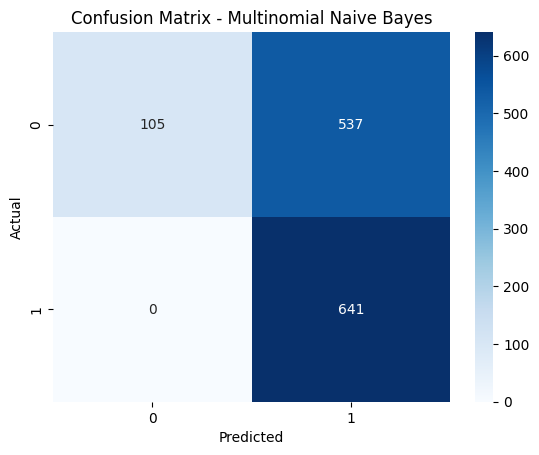
\includegraphics[width=0.6\textwidth,height=0.6\textheight, keepaspectratio]{figures/hyperparam/MNB_default.png}
        \caption{Confusion Matrix of Multinomial Naive Bayes without Grid Search}
        \label{MNB_default}
\end{figure}

As shown in the confusion matrix of \textbf{Logistic Regression} at \ref{LR_default} the model misclassifies 42 fake news as real news and 51 real news as fake news. It yields an accuracy of approximately 0.93. It has a high recll for class 1 and 0 at both 0.93 and 0.92 respectively. The f1-score for both class 1 and 0 are 0.93.

\begin{figure}[h!]
    \centering
    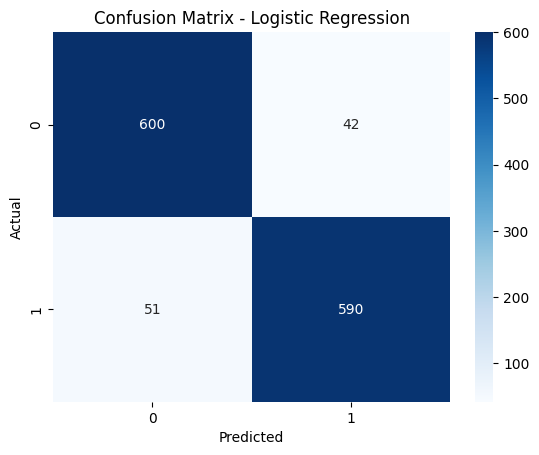
\includegraphics[width=0.6\textwidth,height=0.6\textheight, keepaspectratio]{figures/hyperparam/LR_default.png}
        \caption{Confusion Matrix of Logistic Regression without Grid Search}
        \label{LR_default}
\end{figure}

\ref{RF_default} depicts the confusion matrix of \textbf{Random Forest}. The model misclassifies 66 fake news and 59 real news. It yields an accuracy of approximately 0.90. It has a recall of 0.90 and 0.91 for class 0 and class 1 respectively. The f1-score of both classes is 0.90 showing balanced metrics.

\begin{figure}[h!]
    \centering
    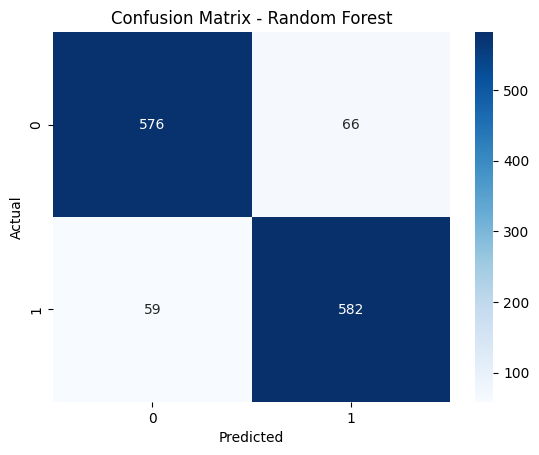
\includegraphics[width=0.6\textwidth,height=0.6\textheight, keepaspectratio]{figures/hyperparam/RF_default.png}
        \caption{Confusion Matrix of Multinomial Naive Bayes without Grid Search}
        \label{RF_default}
\end{figure}

Based on \ref{SVC_default} \textbf{Support Vector Classifier} misclassifies 169 fake news and 70 real news. Thus, it has an accuracy of approximately 0.81. It has a relatively lower recall for class 0 at 0.74. The f1-score for classes 1 and 0 is 0.80 and 0.83 respectively. 

\begin{figure}[h!]
    \centering
    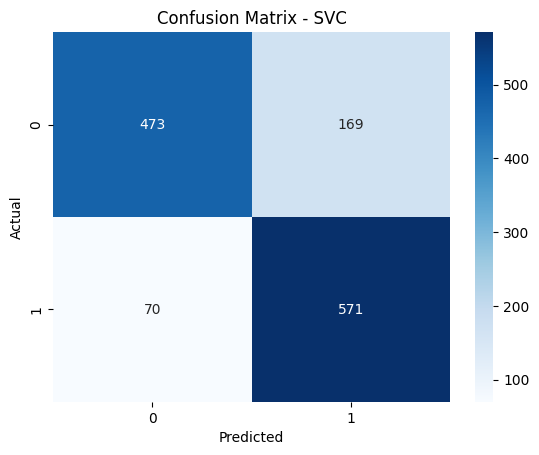
\includegraphics[width=0.6\textwidth,height=0.6\textheight, keepaspectratio]{figures/hyperparam/SVC_default.png}
        \caption{Confusion Matrix of Multinomial Naive Bayes without Grid Search}
        \label{SVC_default}
\end{figure}

Results without hyperparameter tuning are summarized in \ref{tab:no_hyperparam_summary}. AS shown in table \ref{tab:no_hyperparam_summary}, Logistic Regression has the highest F1-Scores while Multinomial Naive Bayes has the lowest.

\begin{table}[ht]
    \centering
    \begin{tabular}{|l|ccc|ccc|}
    \hline
    & \multicolumn{3}{c|}{Multinomial Naive Bayes} & \multicolumn{3}{c|}{Logistic Regression} \\
    \hline
    & Precision & Recall & F1-Score & Precision & Recall & F1-Score \\
    \hline
    Fake & 1.00 & 0.16 & 0.28 & 0.92 & 0.93 & 0.93 \\
    Not Fake & 0.54 & 1.00 & 0.70 & 0.93 & 0.92 & 0.93 \\
    Accuracy & & & 0.58 & & & 0.93 \\
    \hline
    & \multicolumn{3}{c|}{Random Forest} & \multicolumn{3}{c|}{Support Vector Classifier} \\
    \hline
    & Precision & Recall & F1-Score & Precision & Recall & F1-Score \\
    \hline
    Fake & 0.91 & 0.90 & 0.90 & 0.87 & 0.74 & 0.80 \\
    Not Fake & 0.90 & 0.91 & 0.90 & 0.77 & 0.89 & 0.83 \\
    Accuracy & & & 0.90 & & & 0.81 \\
    \hline
    \end{tabular}
    \caption{Performance Metrics for Classifiers with Hyperparameter Tuning}
    \label{tab:no_hyperparam_summary}
\end{table}



\section{Classifiers with Hyperparameter Tuning}
\label{sec:ParamTuning}
To the determine the optimal hyperparameters, all models were tested in the combined dataset using grid search with five-fold cross validation.

Figure \ref{MNB_hyperparam} shows the performance of \textbf{Multinomial Naive Bayes} with an alpha of 0.01 which is the optimal hyperparameter based on the cross validation. The model misclassifies 155 fake news and 18 real news. It yields an accuracy of approximately 0.865. It has the lowest recall for class 0 at 0.87.

\begin{figure}[h!]
\centering
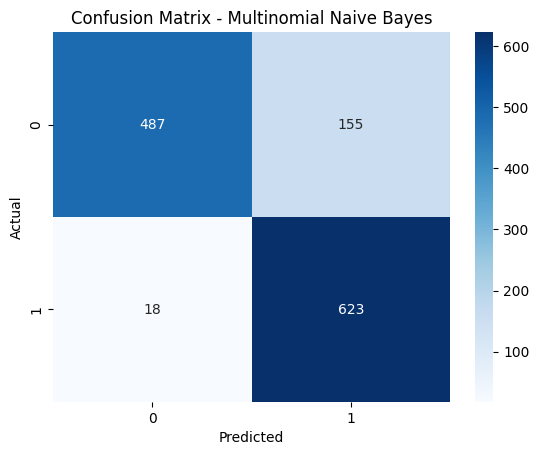
\includegraphics[width=0.6\textwidth,height=0.6\textheight, keepaspectratio]{figures/hyperparam/MNB.png}
    \caption{Confusion Matrix of Multinomial Naive Bayes with alpha = 0.01}
    \label{MNB_hyperparam}
\end{figure}

The best hyperparameter for \textbf{Logistic Regression} is max\_iter = 2000. As shown in \ref{LR_hyperparam} this model misclassified 42 fake news and 51 real news. It yields an accuracy of 0.928 and an F1 score of 0.93 for both class 1 and 0. 

\begin{figure}[h!]
\centering
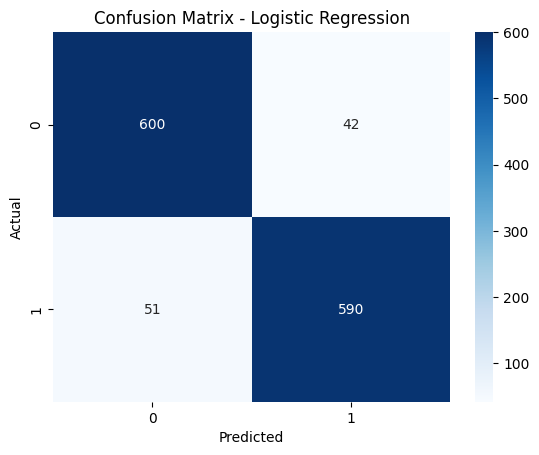
\includegraphics[width=0.6\textwidth,height=0.6\textheight, keepaspectratio]{figures/hyperparam/LR.png}
    \caption{Confusion Matrix of Linear Regression with max\_iter = 2000}
    \label{LR_hyperparam}
\end{figure}

For \textbf{Random Forest}, max\_depth = 20 is the optimal hyperparamter. The performance of this RF is shown in \ref{RF_hyperparam}. The model misclassified 80 fake news and 63 real news. It yields an accuracy of 0.889 with an F1 score of 0.89 for both class 1 and 0.

\begin{figure}[h!]
\centering
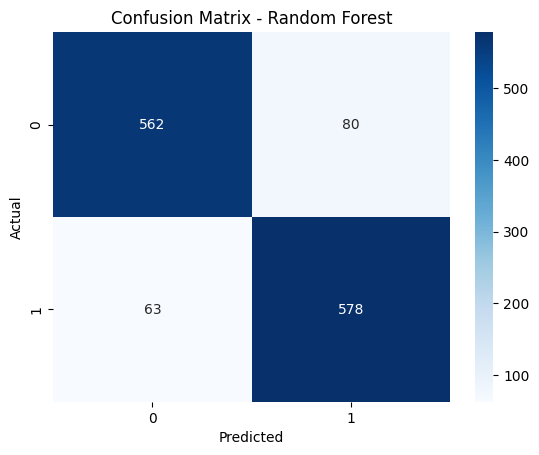
\includegraphics[width=0.6\textwidth,height=0.6\textheight, keepaspectratio]{figures/hyperparam/RF.png}
    \caption{Confusion Matrix of Random Forest with max\_depth = 20}
    \label{RF_hyperparam}
\end{figure}

Lastly, for the \textbf{Support Vector Classifier}, the optimal hyperparameters is C = 0.1 with a linear kernel. As shown in \ref{SVC_hyperparam}, miscclassified 42 fake news and 51 real news. It yields an accuracy of 0.928 and an F1 score of 0.93 for both class 0 and 1. Both the SVC and LR have the highest accuracy during hyperparameter tuning.

\begin{figure}[h!]
\centering
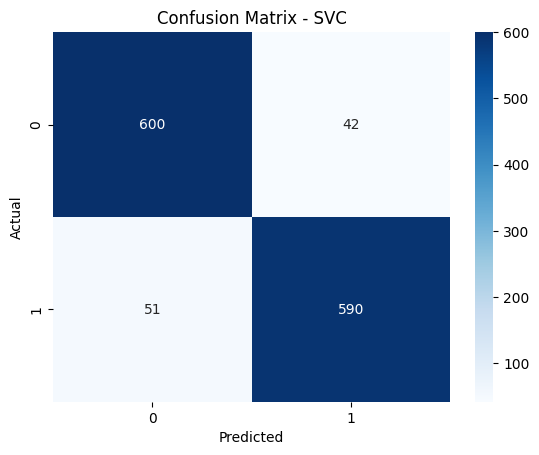
\includegraphics[width=0.6\textwidth,height=0.6\textheight, keepaspectratio]{figures/hyperparam/SVC.png}
    \caption{Confusion Support Vector Classifier with a linear kernel and C = 0.1}
    \label{SVC_hyperparam}
\end{figure}

The results are summarized in table \ref{tab:hyperparam_summary}. Both Logistic Regression and Support Vector Classifier has the highest F1-Scores while Random Forest has the lowest. Comparing the accuracies of the classifiers without hyperparameter tuning in \ref{tab:no_hyperparam_summary} with their accuracies with hyperparameter tuning in \ref{tab:hyperparam_summary}, we can say that hyperparameter tuning significantly increased the accuracy of Multinomial Naive Bayes and Support Vector Classfier, however it did not have any significant impact on the accuracy of Logistic Regression and Random Forest.

\begin{table}[ht]
    \centering
    \begin{tabular}{|l|ccc|ccc|}
    \hline
    & \multicolumn{3}{c|}{Multinomial Naive Bayes} & \multicolumn{3}{c|}{Logistic Regression} \\
    \hline
    & Precision & Recall & F1-Score & Precision & Recall & F1-Score \\
    \hline
    Fake & 0.93 & 0.76 & 0.85 & 0.92 & 0.93 & 0.93 \\
    Not Fake & 0.80 & 0.97 & 0.88 & 0.93 & 0.92 & 0.93 \\
    Accuracy & & & 0.87 & & & 0.93 \\
    \hline
    & \multicolumn{3}{c|}{Random Forest} & \multicolumn{3}{c|}{Support Vector Classifier} \\
    \hline
    & Precision & Recall & F1-Score & Precision & Recall & F1-Score \\
    \hline
    Fake & 0.90 & 0.88 & 0.89 & 0.92 & 0.93 & 0.93 \\
    Not Fake & 0.88 & 0.90 & 0.89 & 0.93 & 0.92 & 0.93 \\
    Accuracy & & & 0.89 & & & 0.93 \\
    \hline
    \end{tabular}
    \caption{Performance Metrics for Classifiers with Hyperparameter Tuning}
    \label{tab:hyperparam_summary}
\end{table}
    
\section{Testing Accuracies}
Using the determined optimal hyperparameters in \ref{sec:ParamTuning}, all four models were tested using five-fold cross validation six times, a total of 30 tests, across three datasets: Cruz (2020), Lupac (2024), and the combination of the two datasets. Average accuracies of the models is shown in \ref{tab::AverageAccuracies}. Logistic Regression and Support Vector Classifier have the highest average accuracy tested in Cruz (2020) and Lupac (2024) dataset. For the combined dataset, only Logistic Regression has the highest average accuracy. Compared with other models and compared in other datasets, Multinomial Naive Bayes and Random Forest performed relatively worst in the combined dataset with an accuracy of 86.0\% and 88.8\% respectively. \ref{tab::AverageAccuracies} shows the average accuracies of the models and the box plot of the accuracies across is depicted in \ref{fig:box_plot_accuracy}.

\begin{tabularx}{\textwidth}{|l|l|c|}
    \hline Classifier & Dataset & Average Accuracy \\ \hline
    \endfirsthead

    \hline
    \multicolumn{3}{|r|}
    {Continued from previous page.} \\
    \hline
    Classifier  & Dataset & Average Accuracy \\ \hline
    \endhead

    \hline \multicolumn{3}{|r|}{{Continued on next page...}} \\ \hline
    \endfoot
    
    \hline
    \caption{Average Accuracies}
    \endlastfoot

    Logistic Regression & Cruz & 0.951 \\
    & Lupac & 0.947\\
    & Combined & 0.924 \\
    \hline
    Multinomial Naive Bayes & Cruz & 0.923 \\
    & Lupac & 0.885 \\
    & Combined & 0.860 \\
    \hline
    Random Forest & Cruz & 0.919 \\
    & Lupac & 0.926 \\
    & Combined & 0.888 \\  
    \hline
    Support Vector Classifier & Cruz & 0.951 \\
    & Lupac & 0.947 \\
    & Combined & 0.922
\label{tab::AverageAccuracies}
\end{tabularx}

\begin{figure}[h!]
    \centering
    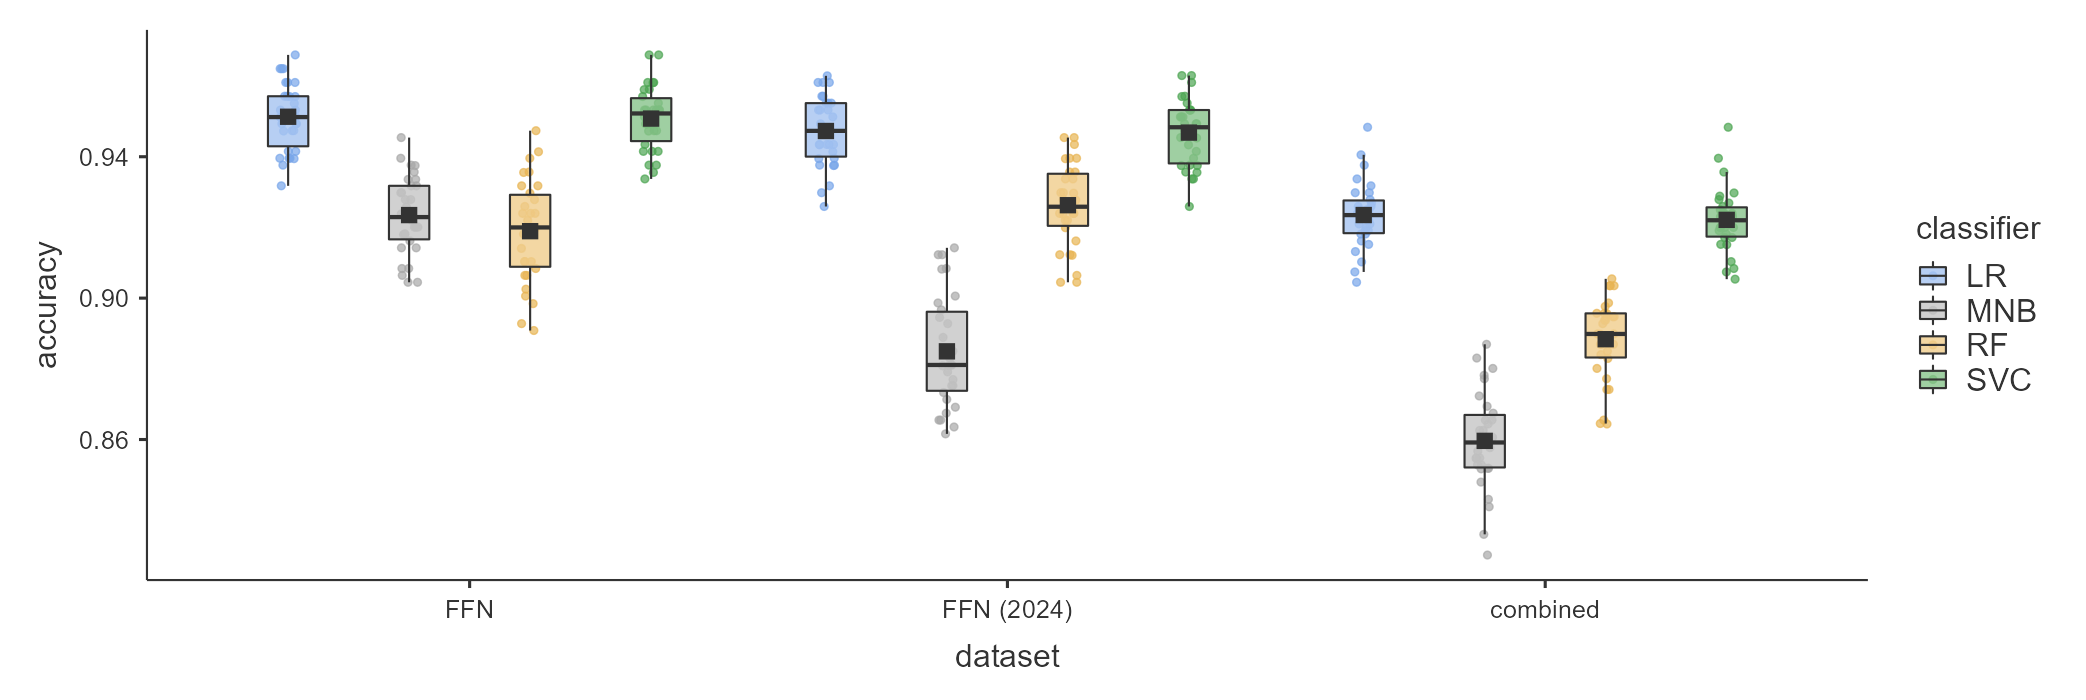
\includegraphics[width=\textwidth,height=\textheight, keepaspectratio]{figures/stats/box_plot.png}
        \caption{Box plot of the accuracies accross datasets}
        \label{fig:box_plot_accuracy}
\end{figure}

Shapiro-Wilk test of normality was used to assess the normality of each group in a two-way layout, where accuracies is the dependent variable and dataset and classfiers are the factors. As shown in table \ref{tab::normality_tests} all groups have p-values greater than of equal to 0.05 indicating the the data is normaly distributed in the two-way layout. However, with a p-value (0.003) lower than 0.05, Levene's homogeneity Test determined the variances of the groups to be heterogenous.

\begin{tabularx}{\textwidth}{|l|l|l|l|}
    \hline
    Dataset & Classfier & Statistic & p-value \\
    \hline
    Cruz & LR & 0.968 & 0.492 \\
    & MNB & 0.971 & 0.571 \\
    & RF & 0.985 & 0.938 \\
    & SVC & 0.972 & 0.603 \\
    \hline
    Lupac & LR & 0.963 & 0.363 \\
    & MNB & 0.940 & 0.928 \\
    & RF & 0.962 & 0.342 \\
    & SVC & 0.972 & 0.598 \\
    \hline
    Combined & LR & 0.979 & 0.793 \\
    & MNB & 0.981 & 0.852 \\
    & RF & 0.934 & 0.063 \\
    & SVC & 0.950 & 0.164 \\
    \hline
\caption{Shapiro-Wilk normality test}
\label{tab::normality_tests}
\end{tabularx}

To determine if there are significant differeces between accuracies of different classifiers in different datasets and taking into account the heteroscedacity of the data, the two-way ANOVA for trimmed means was performed. As shown in Table \ref{tab::two-way} there is a significant difference (p-value = 0.001) between accuracies in different datasets averaged across the classifers. Additionally, there is a significant difference (p-value = 0.001) between accuracies in the classfiers averaged across the datasets. Furthermore, their interaction effect is also significant (p-value = 0.001). Thus, accuracy is affected both by the main effects of the dataset and classfier and also their combinations.

\begin{tabularx}{\textwidth}{|l|l|l|}
    \hline
    Factor & Statistic & p-value \\
    \hline
    dataset & 689.45 & 0.001 \\
    \hline
    classfier & 1010.0371 & 0.001 \\
    \hline
    dataset*classfier & 129.07 & 0.001 \\
    \hline
\caption{Two-way ANOVA for Trimmed Means}
\label{tab::two-way}
\end{tabularx}

To determine which specific subgroups of have significant differeces, pot-hoc mean-separation testing is conducted using Bonferroni correction for subgroups of each dataset level. As shown in Table \ref{tab::post-hoc} the only subgroups that do not have significant differences are Logistic Regression and Support Vector Classfier accross all datasets, and Multinomial Naive Bayes and Random Forest in the Cruz (2020) dataset. The results is reflected in the interaction plot of the accuracies at Figure \ref{fig:interaction_plot} As show in Figure \ref{fig:interaction_plot} accuracies of Logistic Regression and Support Vector Classfier are almost equal across all datasets. The same can be said for the accuracy of Multinomial Naive Bayes and Random Forest in the Cruz (2020) dataset.

\begin{tabularx}{\textwidth}{|l|l|l|l|}
    \hline Dataset & Classfier (a) & Classfier(b) & p-value \\ \hline
    \endfirsthead

    \hline
    \multicolumn{3}{|r|}
    {Continued from previous page.} \\
    \hline
    Classifier  & Dataset & Average Accuracy \\ \hline
    \endhead

    \hline \multicolumn{3}{|r|}{{Continued on next page...}} \\ \hline
    \endfoot
    
    \hline
    \caption{Bonferroni correction for subgroups of each data level}
    \endlastfoot

    Cruz & LR & MNB & \textless 0.001 \\
    \cline{3-4}
    & & RF & \textless 0.001 \\
    \cline{3-4}
    & & SVC & 1.00 \\
    \cline{2-4}
    & MNB & RF & 1.00 \\
    \cline{3-4}
    & & SVC & \textless 0.001 \\
    \cline{2-4}
    & RF & SVC &  \textless 0.001 \\
    \hline
    Lupac & LR & MNB & \textless 0.001 \\
    \cline{3-4}
    & & RF & \textless 0.001 \\
    \cline{3-4}
    & & SVC & 1.00 \\
    \cline{2-4}
    & MNB & RF & \textless 0.001 \\
    \cline{3-4}
    & & SVC & \textless 0.001 \\
    \cline{2-4}
    & RF & SVC &  \textless 0.001 \\
    \hline
    Combined & LR & MNB & \textless 0.001 \\
    \cline{3-4}
    & & RF & \textless 0.001 \\
    \cline{3-4}
    & & SVC & 1.00 \\
    \cline{2-4}
    & MNB & RF & \textless 0.001 \\
    \cline{3-4}
    & & SVC & \textless 0.001 \\
    \cline{2-4}
    & RF & SVC &  \textless 0.001
\label{tab::post-hoc}
\end{tabularx}

\begin{figure}[h!]
    \centering
    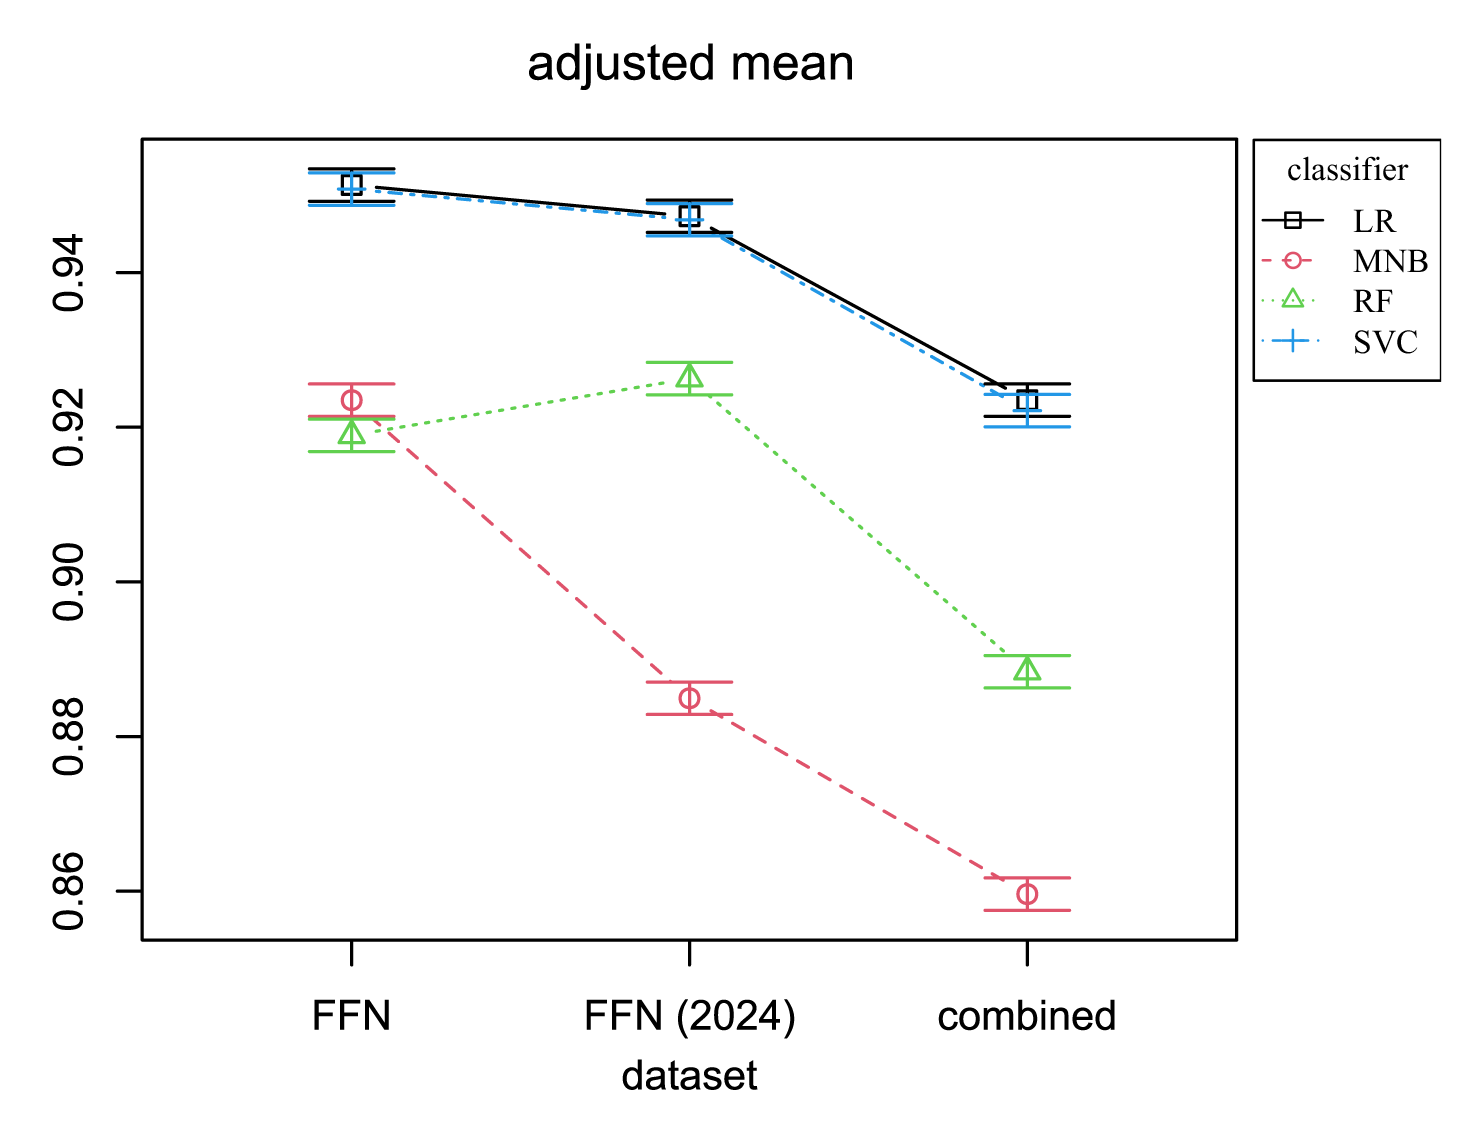
\includegraphics[width=\textwidth,height=\textheight, keepaspectratio]{figures/stats/im.png}
        \caption{interaction plot of accuracies accross datasets}
        \label{fig:interaction_plot}
\end{figure}


% Shapiro-Wilk test of normality was used for accuracies accross datasets. With a p-value (\textless 0.001) lower than 0.05, the data is determine to be not normaly distributed, thus the non-parameteric Kruskal-Wallis test was used to check if the differences between the accuracies accross datasets are significant. 

% The p-value (\textless 0.001) corresponding to the test-statistic of Kruskal-Wallis test is lower than 0.05 which suggests that one or more differeces in accuracies accross datasets are significant. Dwass-Steel-Critchlow-Fligner (DSCF) pariwise comparisons for post-hoc test showed that the differences in accuracies between Cruz (2020) and the combined dataset, and Lupac (2024) and the combined dataset are significant. Therefore, at least one classifier performed significantly better on the Cruz (2020) and Lupac (2024) dataset compared with their performance on the combined dataset. See \ref{tab::dscf_datasets} for the results of the DSCF pairwise comparisons. To deter

% \begin{tabularx}{\textwidth}{|l|c|c|}
%     \hline
%     & W & p \\
%     \hline
%     Cruz - Lupac & -2.91 & 0.099 \\
%     \hline
%     Cruz - Combined & -13.67 &  \textless 0.001 \\
%     \hline
%     Lupac - Combined & -10.37 & \textless 0.001\\
%     \hline
% \caption{DSCF pairwise comparisons across datasets}
% \label{tab::dscf_datasets}
% \end{tabularx}

% For accuracies across classifers, Shapiro-Wilk was used and it was determined that the data is normality distributed (p-value = 0.152). However, using Levene's test for homogeneity of variances showed that the data does not have equal vairances. Thus Kruskal-Wallis test was used to check if the differences between accuracies accross classfiers are significant.

% The p-value (\textless 0.001) of the Kruskal-Wallis test is less than 0.05 suggesting that at least one difference between accuracies accross classfiers is significant. Results of DSCF pairwise comparisons showed that all pairs of classifiers have significant differences except for Logistic Regression and Support Vector Classifier. Table \ref{tab::dscf_classifiers} shows the results of DSCF pairwaise comparisons. Based on table \ref{tab::dscf_classifiers}, LR and SVC performed significantly better compared to MNB and RF, and RF permored better than MNB. Thus, the classifiers with the best to worst accuracy would be LR, SVC, RF, then MNB with LR and SVC having no significant difference.

% \begin{tabularx}{\textwidth}{|l|c|c|}
%     \hline
%     & W & p \\
%     \hline
%     LR - MNB & -14.217 & \textless 0.001 \\
%     \hline
%     LR - RF & -12.0.2 &  \textless 0.001 \\
%     \hline
%     LR - SVC & -0.56 & 0.979\\
%     \hline
%     MNB - RF & 7.025 & \textless 0.001 \\
%     \hline
%     MNB - SVC & 14.064  & \textless 0.001 \\
%     \hline
%     RF - SVC & 11.755 & \textless 0.001 \\
%     \hline
% \caption{DSCF pairwise comparisons across classifiers}
% \label{tab::dscf_classifiers}
% \end{tabularx}